\documentclass[border=6pt]{standalone}
\usepackage{tikz}
\usetikzlibrary{positioning}

% Colours approximating the original figure
\definecolor{nodefill}{RGB}{245,230,150}  % goldenrod / khaki
\definecolor{nodeline}{RGB}{40,40,120}     % navy
\definecolor{numcol}{RGB}{200,40,40}       % red preorder numbers

\begin{document}
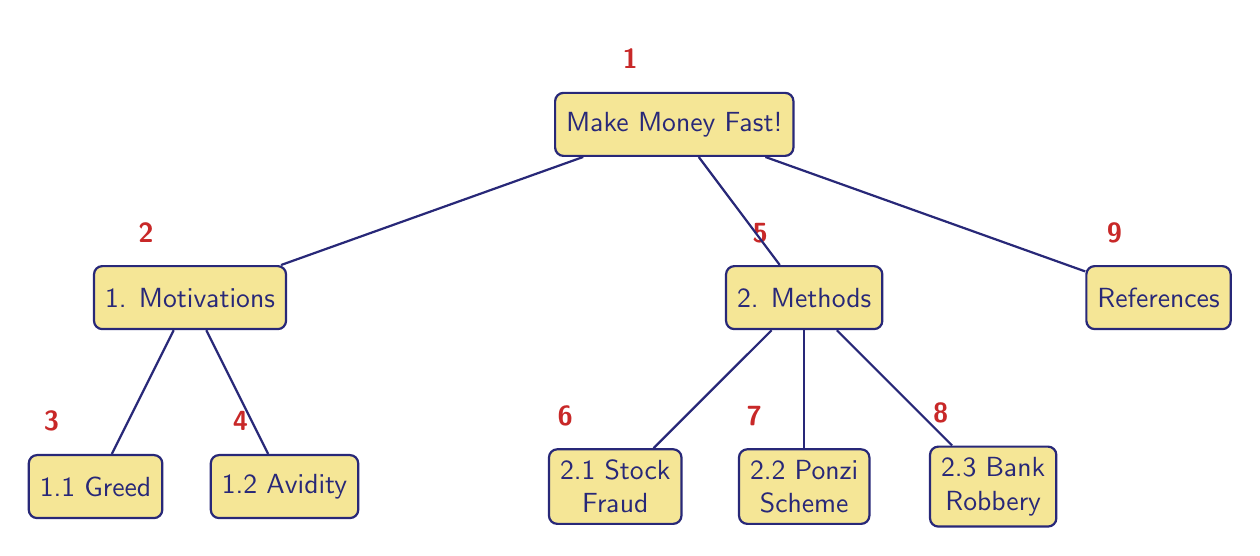
\begin{tikzpicture}[
  font=\sffamily,
  every node/.style={
    draw=nodeline, line width=0.8pt, rounded corners=3pt,
    fill=nodefill, text=nodeline, align=center,
    inner sep=4pt, minimum height=8mm
  },
  num/.style={
    draw=none, fill=none, text=numcol, font=\sffamily\bfseries,
    inner sep=1pt
  },
  edge/.style={draw=nodeline, line width=0.8pt},
]

% ---- Nodes (preorder number given as an above-left label) ----
\node (root)  at (1.35, 0)    [label={[num]above left:1}] {Make Money Fast!};

\node (mot)   at (-4.8,-2.2)  [label={[num]above left:2}] {1. Motivations};
\node (met)   at ( 3.0,-2.2)  [label={[num]above left:5}] {2. Methods};
\node (ref)   at ( 7.5,-2.2)  [label={[num]above left:9}] {References};

\node (greed) at (-6.0,-4.6)  [label={[num]above left:3}] {1.1 Greed};
\node (avid)  at (-3.6,-4.6)  [label={[num]above left:4}] {1.2 Avidity};

\node (stock) at ( 0.6,-4.6)  [label={[num]above left:6}] {2.1 Stock\\Fraud};
\node (ponzi) at ( 3.0,-4.6)  [label={[num]above left:7}] {2.2 Ponzi\\Scheme};
\node (bank)  at ( 5.4,-4.6)  [label={[num]above left:8}] {2.3 Bank\\Robbery};

% ---- Edges ----
\foreach \p/\c in {root/mot, root/met, root/ref,
                   mot/greed, mot/avid,
                   met/stock, met/ponzi, met/bank}
  \draw[edge] (\p) -- (\c);

\end{tikzpicture}
\end{document}
